\chapter{Results}

{\color{red}If I ever get any results go in here.}

\section{Magneto-Optic Trap Analysis}

\subsection{Temperature}
Knowing the temperature of the \gls{mot} allows optimisation of the parameters of the \gls{odt} and can be useful for optimising the \gls{mot} itself.

The procedure for calculating the temperature was discussed in section \ref{temp_measurement}. The data for this measurement was collected by releasing the \gls{mot}, waiting for a number of milliseconds and them imaging the cloud.

A python program was written to analyse this data. A two dimentional, elliptical Gaussian distribution was fitted to each of the images. The 1/e radius of each of these distributions was used to fit to equation \ref{eq:cloud_radius} and the temperature was calculated with equation \ref{eq:temp_velocity}. The results of this program are shown in figure \ref{fig:temp_fits}.

\begin{figure}[h]
\begin{subfigure}[b]{0.5\textwidth}
    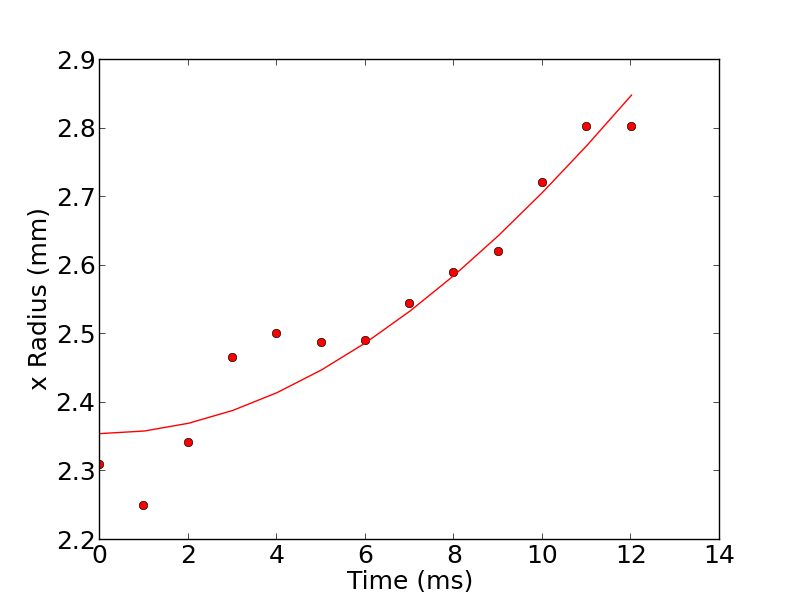
\includegraphics[width=\textwidth]{figs/final_temp_fitting_x.png}
\end{subfigure}\begin{subfigure}[b]{0.5\textwidth}
    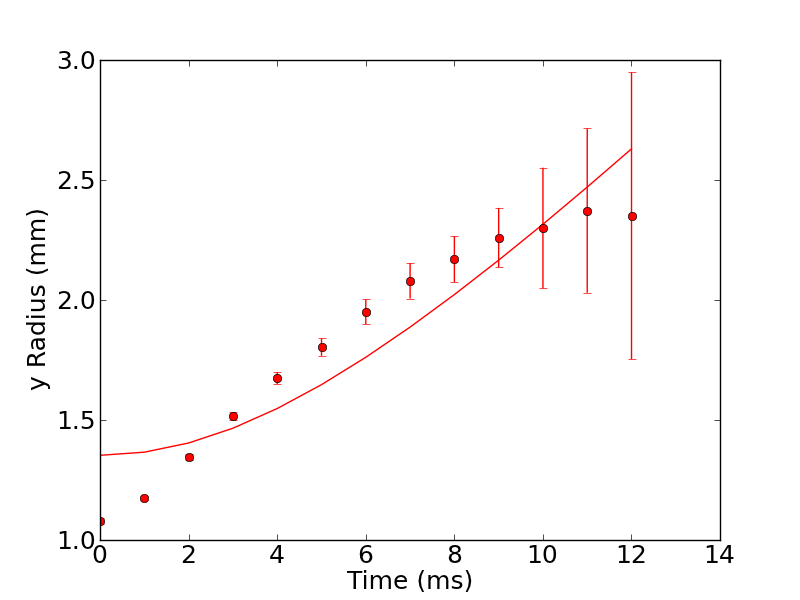
\includegraphics[width=\textwidth]{figs/final_temp_fitting_y.png}
\end{subfigure}
\caption{Data of thermal expansion of the MOT (red dots) and the fitted curve (red line).}
\label{fig:temp_fits}
\end{figure}

The temperature of the \gls{mot} was determined to be $139\,\unit{\mu K}$ which is close to the previously measured temperature of $70\,\unit{\mu K}$. Since the previous measurement was made the detuning on the \gls{mot} cooling beams has been increase to optimise the loading rate which would explain the increase in temperature.

\subsection{Atom Count}
\label{mot_atom_count}
The number of atoms is the \gls{mot} is another useful metric. The number of atoms in the \gls{mot} can be compared to the number in the \gls{odt} and the number in similar \glspl{mot} .

The theory involved in this calculation is discussed in section \ref{atom_count}. The imaging laser is well above the saturation intensity in the centre beam so equation \ref{eq:atom_count} must be used.

Another python program was used to perform this calculation on the same data that was used for the temperature measurements. As expected the number of atoms in each of the images remains constant until the edges of the cloud reach the limits of the \gls{ccd} as you can see in figure \ref{fig:mot_atom_count}. The number of atoms in the \gls{mot} is therefore $1.3 \pm0.19\times10^8$ which is comparable to measurements made previously with the \gls{caes}\cite{sheludko_shaped_2010}.

\begin{figure}
\centering
    \begin{subfigure}[b]{0.3\textwidth}
    \centering
    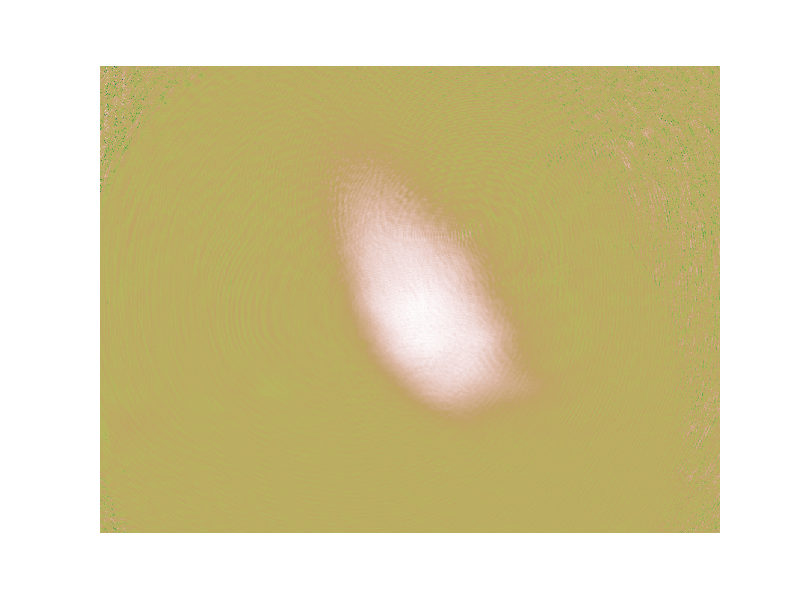
\includegraphics[width=\textwidth]{figs/MOTimage1.png}
    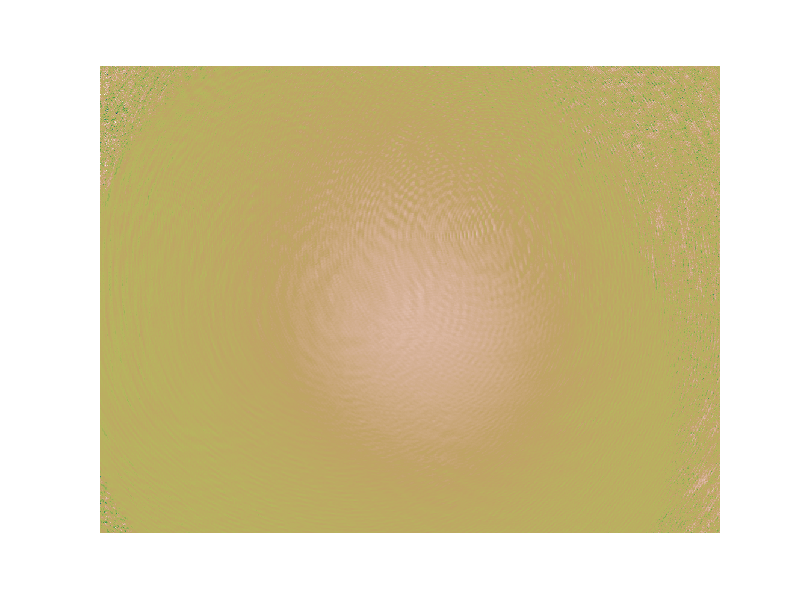
\includegraphics[width=\textwidth]{figs/MOTimage2.png}
    \caption{The MOT $1\,\unit{ms}$ (top) and $9\,\unit{ms}$ (bottom) after release.}
    \end{subfigure}~~~\begin{subfigure}[b]{0.6\textwidth}
    \centering
    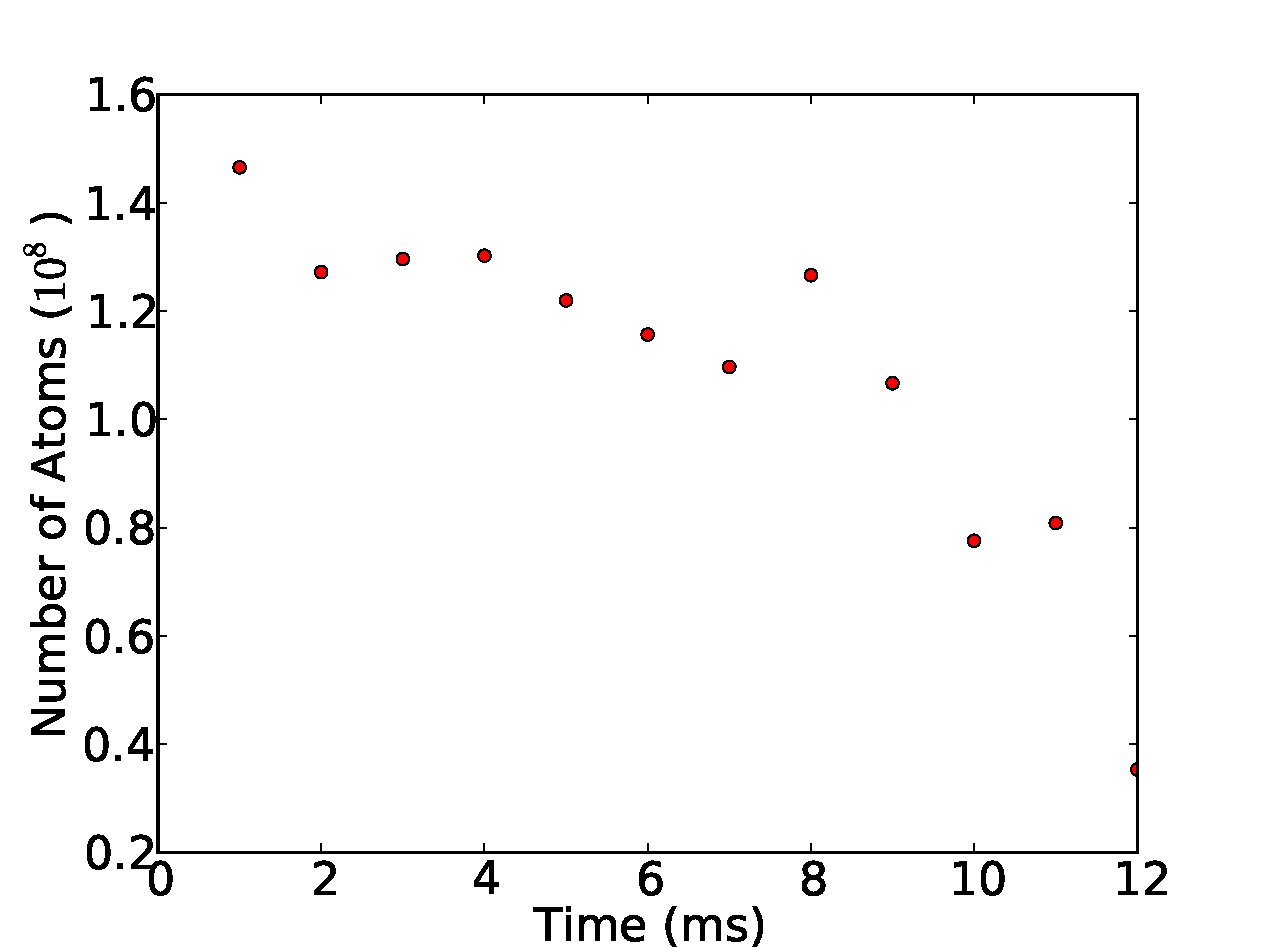
\includegraphics[width=\textwidth]{figs/MOT_atom_count.pdf}
    \caption{The evolution of the number of atoms imaged by the camera after release.}
    \label{fig:mot_atom_count}
    \end{subfigure}
    \caption{}
\end{figure}

\section{Optical Dipole Trap Analysis}
The first optical dipole trapping was observed in September 2012 and the first crossed \gls{odt} images acquired in early October 2012. Initially trapping along only the first beam of the \gls{odt} was observed despite both beams beaing supposedly aligned. After further alignment and changes to the beam focussing trapping was observed in both beams with no evidence of a region of overlapped traps. Eventually however the beams were properly aligned and crossed trapping was observed as shown in figure \ref{fig:ODTimage1}.

An interesting effect can be observed in the crossed \gls{odt} images. Atoms within the \gls{odt} region can be seen being pushed down the beam by the scattering force of the trapping laser while leaving the core of the \gls{odt} behind. This is shown in figure \ref{fig:crossed_effect}. This effect implies that the \gls{odt} is not deep enough to trap all of the atoms within the trapping region. This can be fixed by either increasing the depth of the \gls{odt} or reducing the temperature of the \gls{mot}.

\begin{figure}
    \centering
    \begin{subfigure}[b]{0.3\textwidth}
        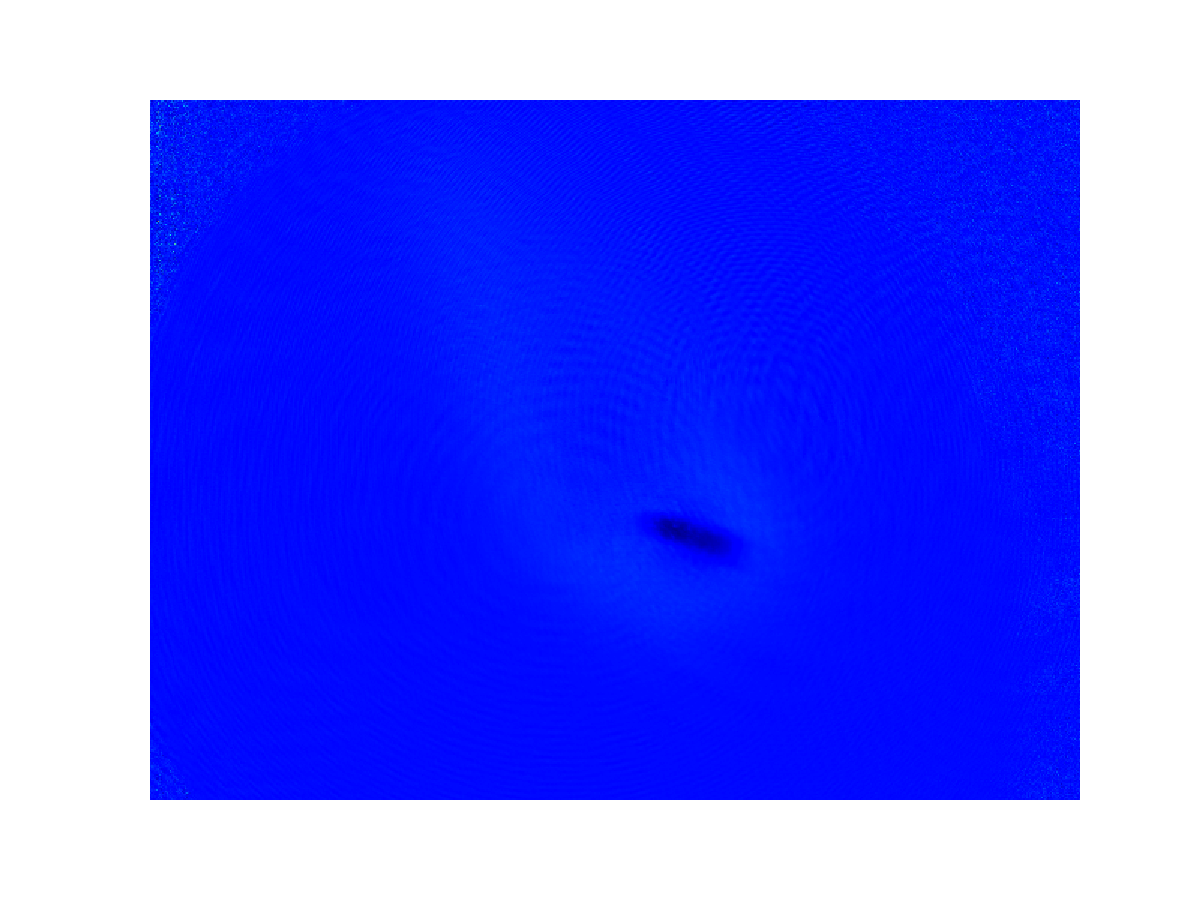
\includegraphics[width=1.1\textwidth]{figs/ODTimage1.pdf}
    \end{subfigure}\begin{subfigure}[b]{0.3\textwidth}
        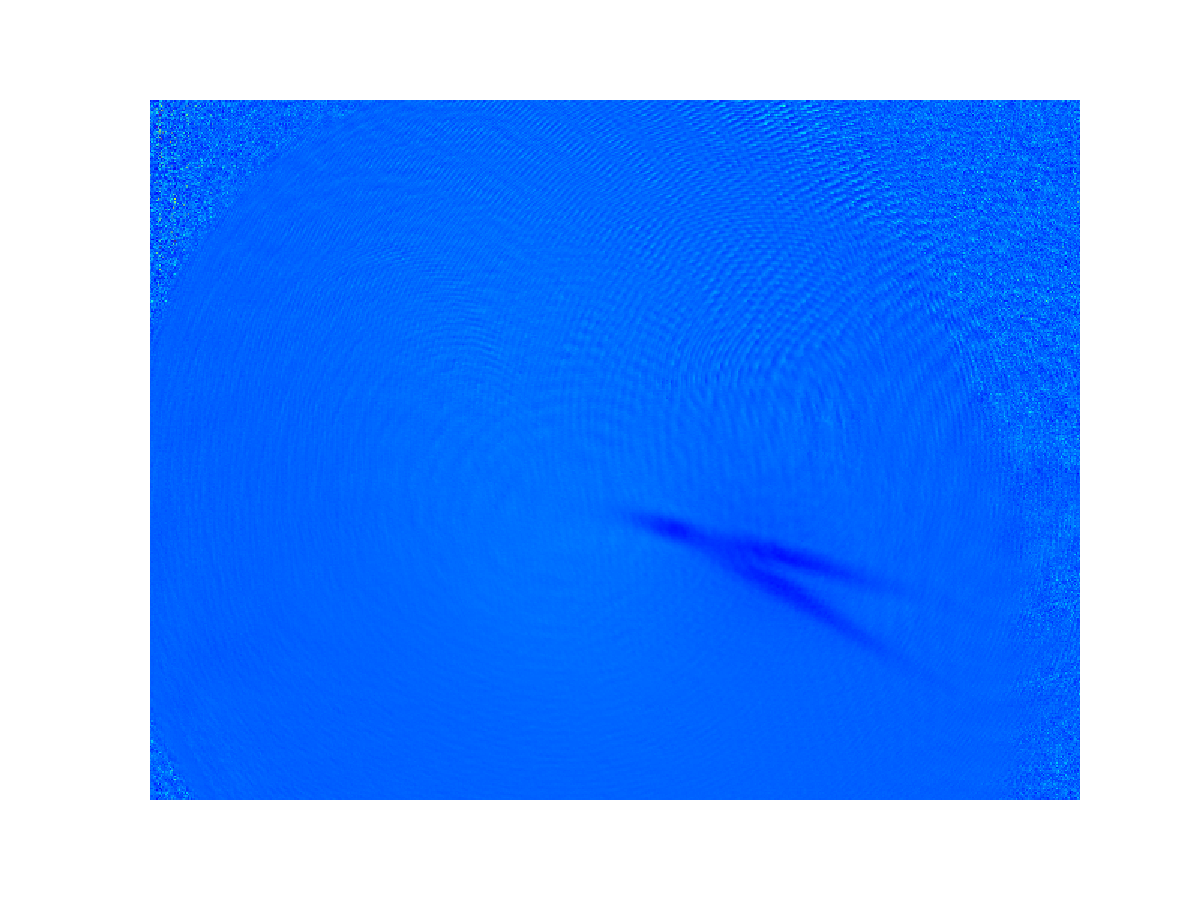
\includegraphics[width=1.1\textwidth]{figs/ODTimage2.pdf}
    \end{subfigure}\begin{subfigure}[b]{0.3\textwidth}
        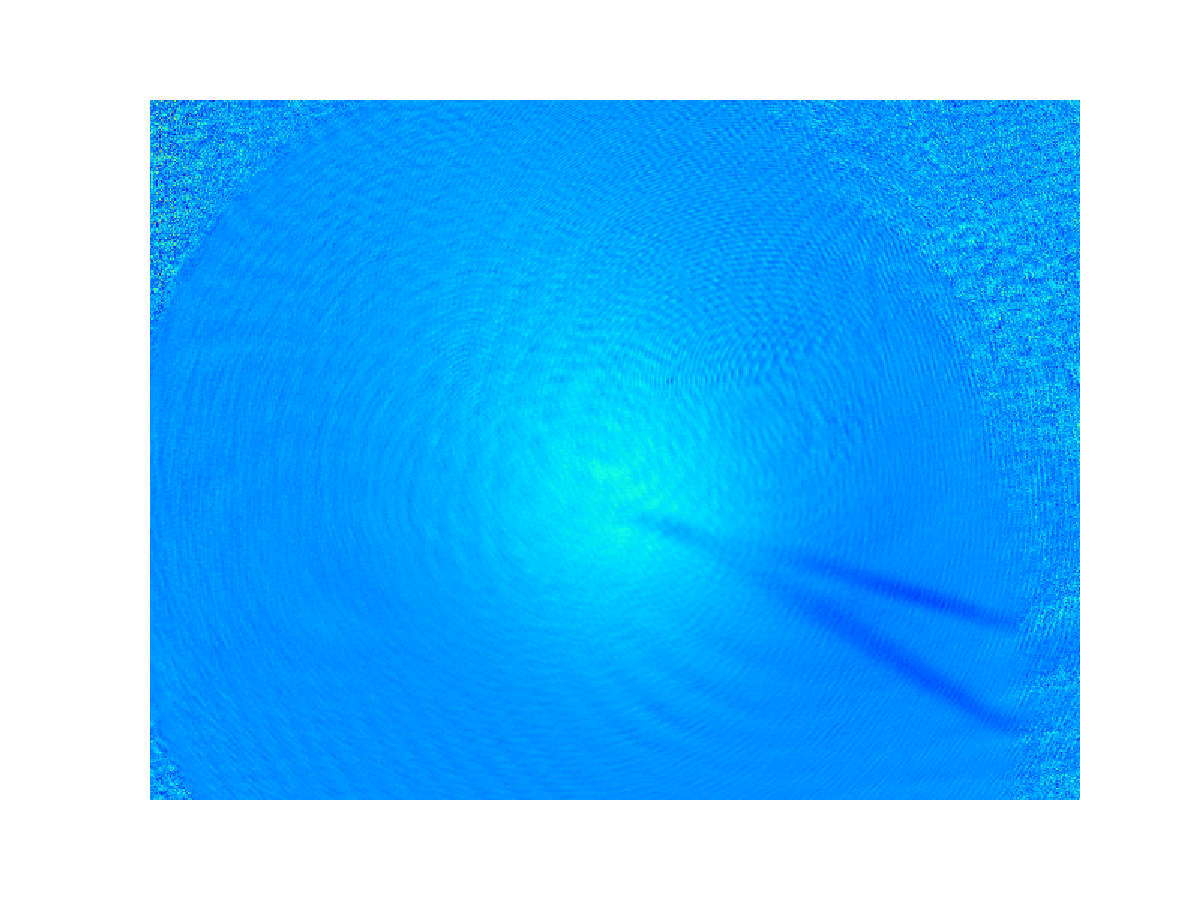
\includegraphics[width=1.1\textwidth]{figs/ODTimage3.pdf}
    \end{subfigure}
\caption{A crossed ODT and untrapped atoms in the region of the ODT being pushed down the trapping beams. The images are taken 2, 4 and $6\,\unit{ms}$ after the MOT trapping has be turned off.}
\label{fig:crossed_effect}
\end{figure}

\subsection{Size}
The size of the crossed \gls{odt} can be calulated by fitting Gaussian curves to the distribution as shown in figure \ref{fig:ODTimage1} and taking the 1/e radius from the fit. Here the 1/e length of the trap was found to be $1292.6\,\unit{\mu m}$ and the width to be $417.4\,\unit{\mu m}$. The \gls{odt} laser was tuned to $\lambda=780.317\,\unit{nm}$ and the \gls{mot} was turned off $2\,\unit{ms}$ before imaging.

\begin{figure}[h]
\centering
    % row 1
    \begin{subfigure}[b]{0.5\textwidth}
        \centering
        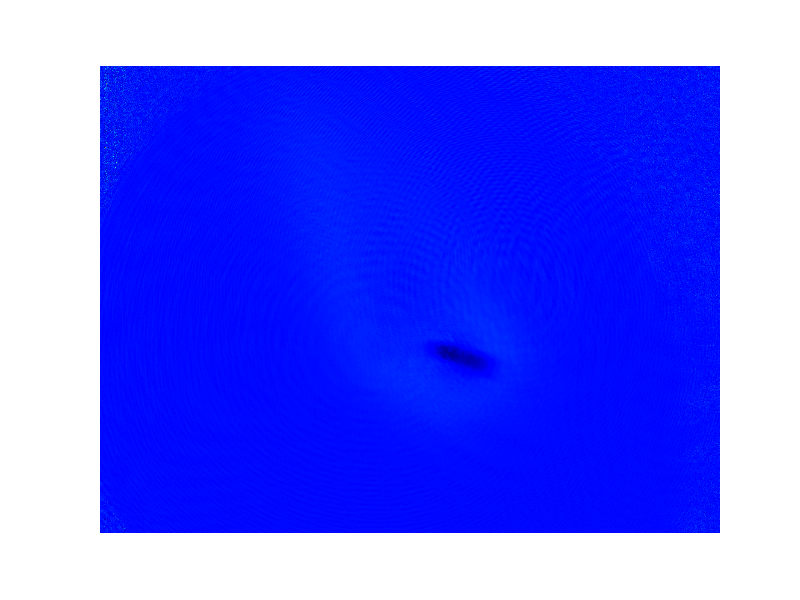
\includegraphics[width=0.8\textwidth]{figs/ODTimage1.png}
        \caption{The crossed ODT.}
    \end{subfigure}\begin{subfigure}[b]{0.5\textwidth}
        \centering
        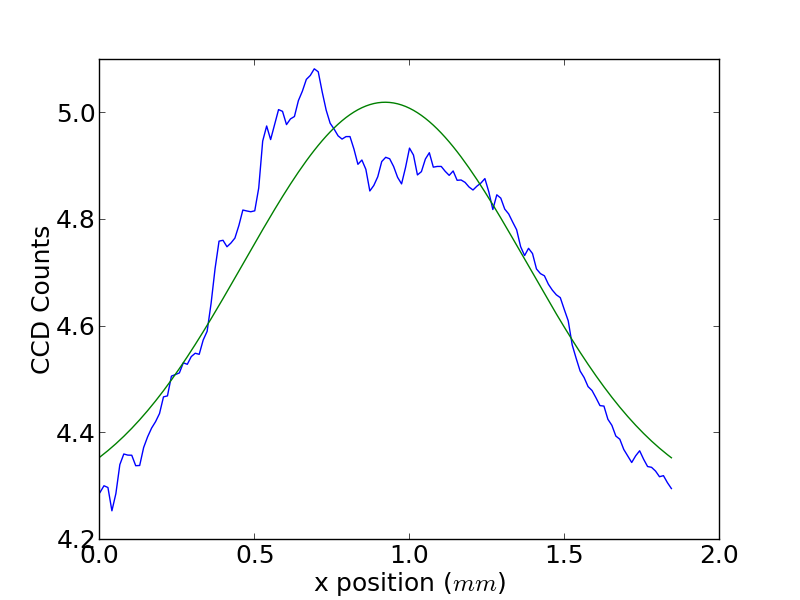
\includegraphics[width=0.8\textwidth]{figs/ODTimage1x.png}
        \caption{Vertical cross-section though the centre of the ODT.}
    \end{subfigure}

    % row 2
    \begin{subfigure}[b]{0.5\textwidth}
        \centering
        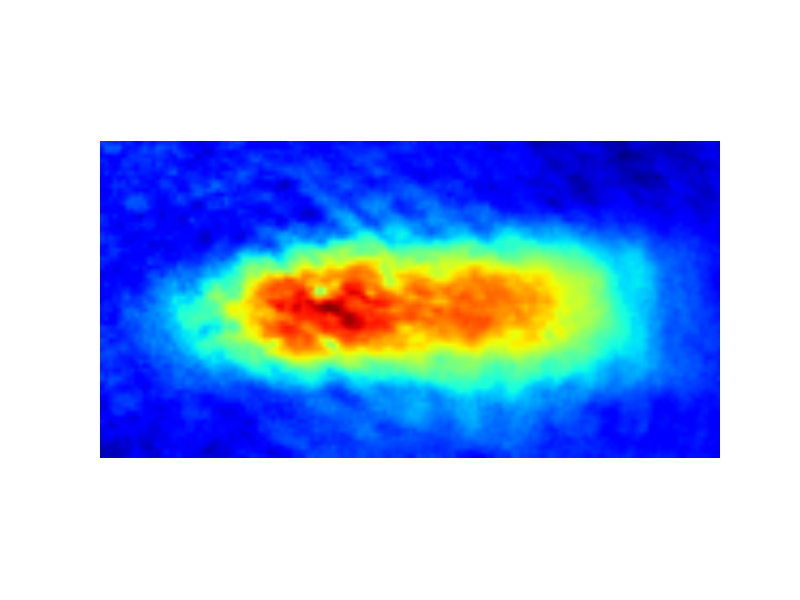
\includegraphics[width=0.9\textwidth]{figs/ODTimage1zoom.png}
        \caption{The crossed ODT in detail.}
    \end{subfigure}\begin{subfigure}[b]{0.5\textwidth}
        \centering
        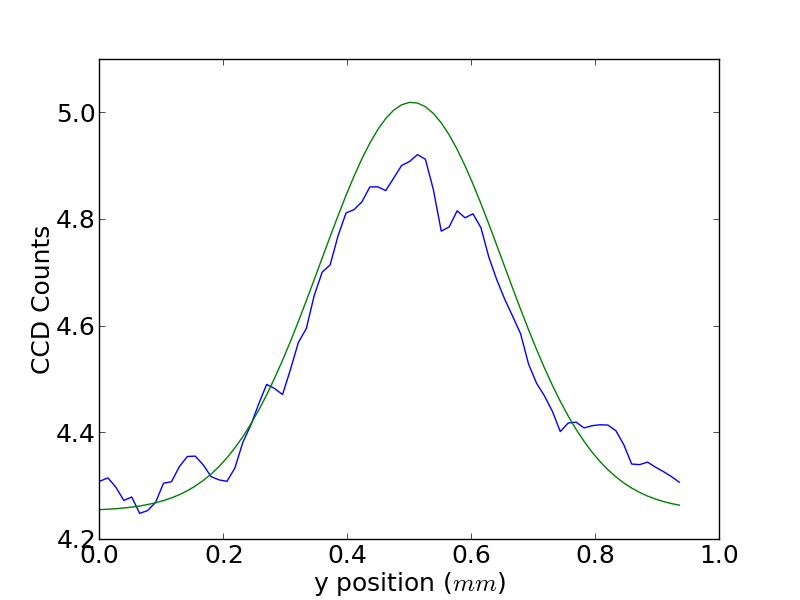
\includegraphics[width=0.8\textwidth]{figs/ODTimage1y.png}
        \caption{Horizontal cross-section through the centre of the ODT.}
    \end{subfigure}

    \caption{}
    \label{fig:ODTimage1}
\end{figure}


\subsection{Atom Count}
This analysis works similarly to that described in section \ref{mot_atom_count}. The only real difference here is that the atom count was calulated twice. Once for the dispersing \gls{mot} only and a second time for the combined dispersing \gls{mot} and \gls{odt}. The difference between these values is the number of atoms in the \gls{odt}. As shown in figure \ref{fig:lifetime} the number of atoms in the dipole trap at t=0 is $6.05\times10^6$ which corresponds to approximately 5\% of the \gls{mot} atoms.

\subsubsection{Lifetime}
The simple model that that was described in section \ref{lifetime_section} has been used to determine the 1/e lifetime of the \gls{odt} which is $2.1\,\unit{ms}$.

\begin{figure}[h]
\centering
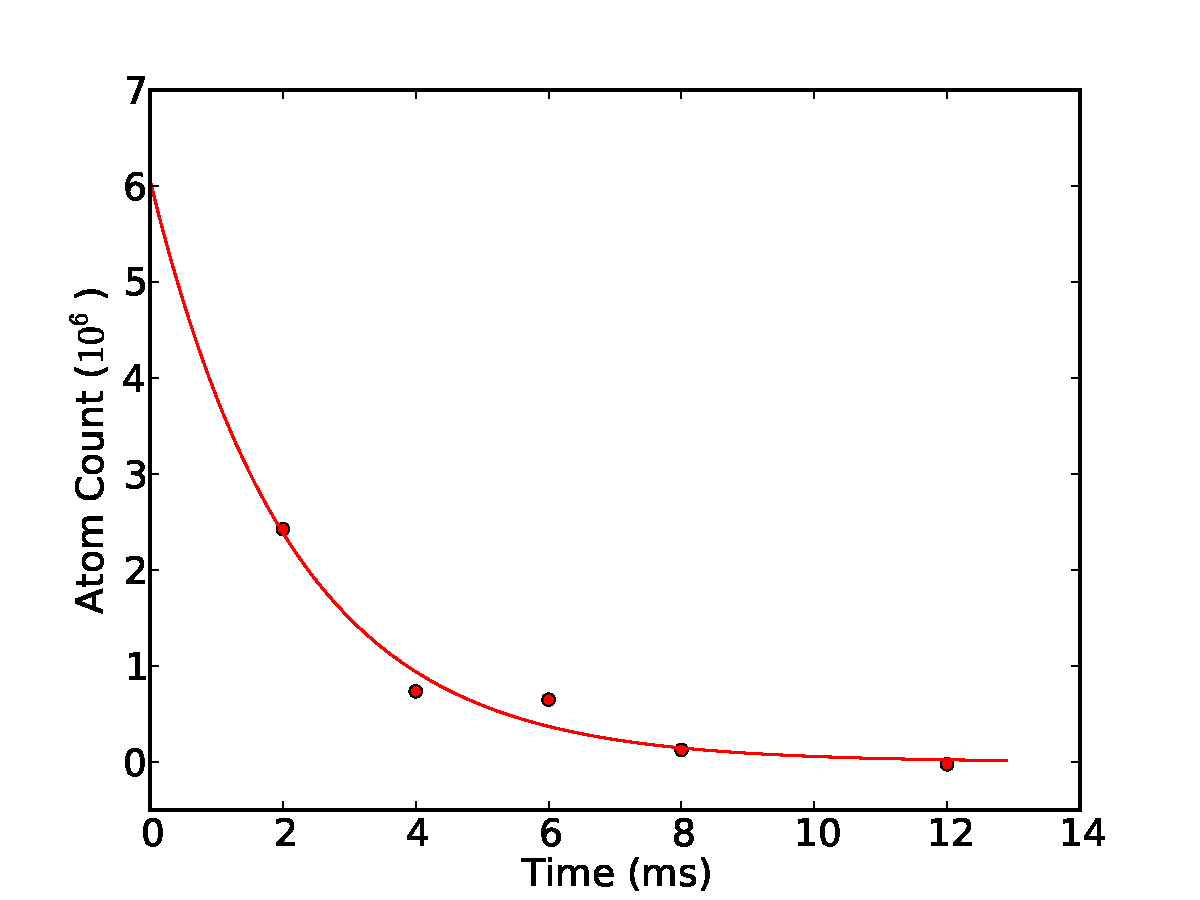
\includegraphics[width=0.5\textwidth]{figs/lifetime.pdf}
\caption{Lifetime of the ODT.}
\label{fig:lifetime}
\end{figure}
